\section{Постановка задачи}
\begin{definition}
	Отклик системы на функцию Хэвисайда называется \definitionfont{переходной характеристикой}.
\end{definition}

\begin{definition}
	Отклик системы на дельта-функцию называется \definitionfont{импульсной функцией}.
\end{definition}

\begin{definition}
	Образ Лапласа $W(s)$ импульсной функции $w(t)$ называется \definitionfont{передаточной функцией} линейной системы.
\end{definition}

\begin{definition}
	Система \definitionfont{устойчива}, если для любой ненулевой ограниченной функции входа, функция выхода ограничена.
\end{definition}

\begin{definition}
	\definitionfont{Ошибкой регулирования} называется функция $e(t) = x(t) - u(t)$, где $x(t)$ --- функция выхода системы, $u(t)$ --- функция входа.
\end{definition}

\begin{definition}
	\definitionfont{Интегральной ошибкой} называется интеграл от модуля ошибки регулирования на интервале наблюдения.
\end{definition}

\begin{definition}
	За показатель \definitionfont{качества регулятора} принимается
	\[\int\limits_{0}^{\infty} |e(\tau)| d \tau\]
\end{definition}

\begin{goal}
	Произвести оптимальную настройку и сравнение П,ПИ и ПИД- регуляторов.
\end{goal}

\begin{tasks}
	\begin{enumerate}
		\item[]
		
		\item Для одноконтурной системы регулирования с ПИ–регулятором определить параметры $K$ и $T_i$ следующими способами:
		\begin{itemize}
			\item покоординатной оптимизацией $K$ и $T_i$ по интегральному критерию качества;
			
			\item по параметрам переходной характеристики объекта.			
		\end{itemize}
		Сравнить полученные системы управления между собой по интегральному критерию качества.
		
		\item Для одноконтурной системы регулирования с ПИД-регулятором определить параметры $K$, $T_i$, $T_d$, $T_s$ следующими способами:
		\begin{itemize}
			\item покоординатной оптимизацией $K$ и $T_i$ по интегральному критерию качества (принять $T_d = T_i / 4$, $T_s = T_d / 8$);
			
			\item по параметрам переходной характеристики объекта.
		\end{itemize}
		Сравнить полученные системы управления между собой по интегральному критерию качества. Сравнить ПИ- и ПИД-регуляторы между собой по интегральному критерию качества исходя из наилучших значений $K$ и $T_i$.
		
		\item Предложить свои формулы настройки параметров ПИД-регулятора исходя из наилучших табличных значений $K$ и $T_i$. Сравнить по интегральному критерию качества регулятор, настроенный по вашим формулам, с регулятором, настроенным по предложенным формулам, для значений параметра задержки объекта $T = 1; 2; 10$.
	\end{enumerate}
\end{tasks}	

\newpage

\section{Порядок выполнения работы}
В ходе работы рассматривались объекты с передаточной функцией\footnote{На схемах вместо $T$ была использована буква $d$}
\[W(s) = \frac{2e^{-sT}}{(1 + T_0 s)^n},\]

а именно --- три объекта: $T = 0; 1.5; 3$, при $T_0 = 1.07$ и $n = 4$. Для каждого из трёх объектов были разработаны П,ПИ,ПИД-регуляторы, построенные в программе MicroCap. В конечном итоге регуляторы были настроены для получения минимальной интегральной ошибки, при этом в качестве функции входа выступала функция $u(t) \equiv 1$.

\begin{figure}[H]
	\centering
	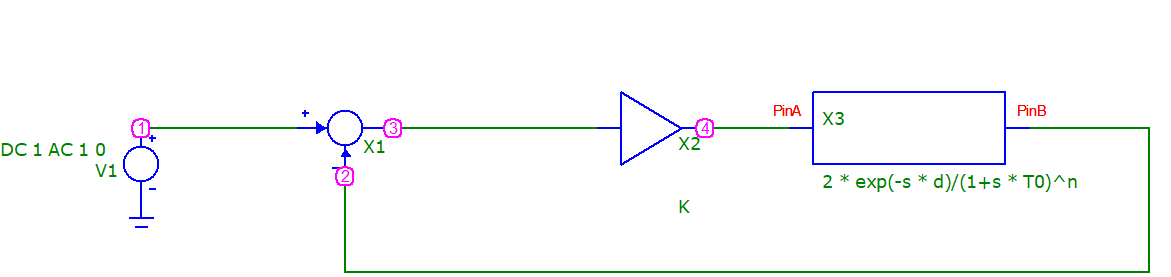
\includegraphics[scale=0.4]{./screens/schemes/p_scheme.png}
	\caption{Схема П-регулятора} 
\end{figure}

\begin{figure}[H]
	\centering
	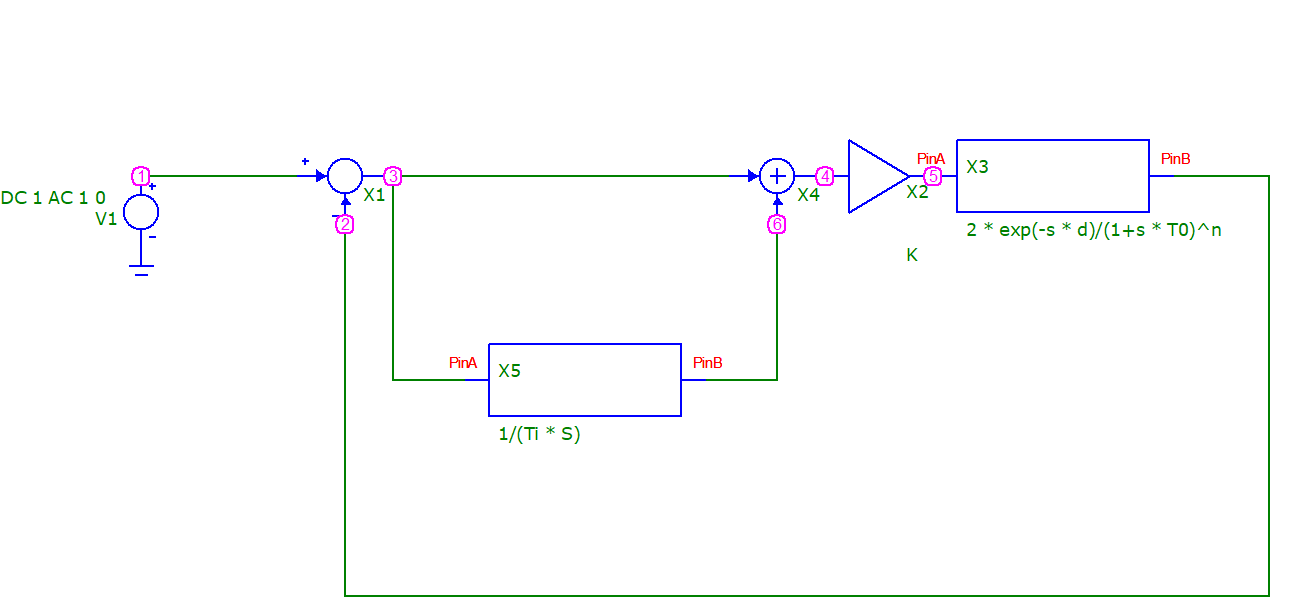
\includegraphics[scale=0.4]{./screens/schemes/pi_scheme.png}
	\caption{Схема ПИ-регулятора} 
\end{figure}

\begin{figure}[H]
	\centering
	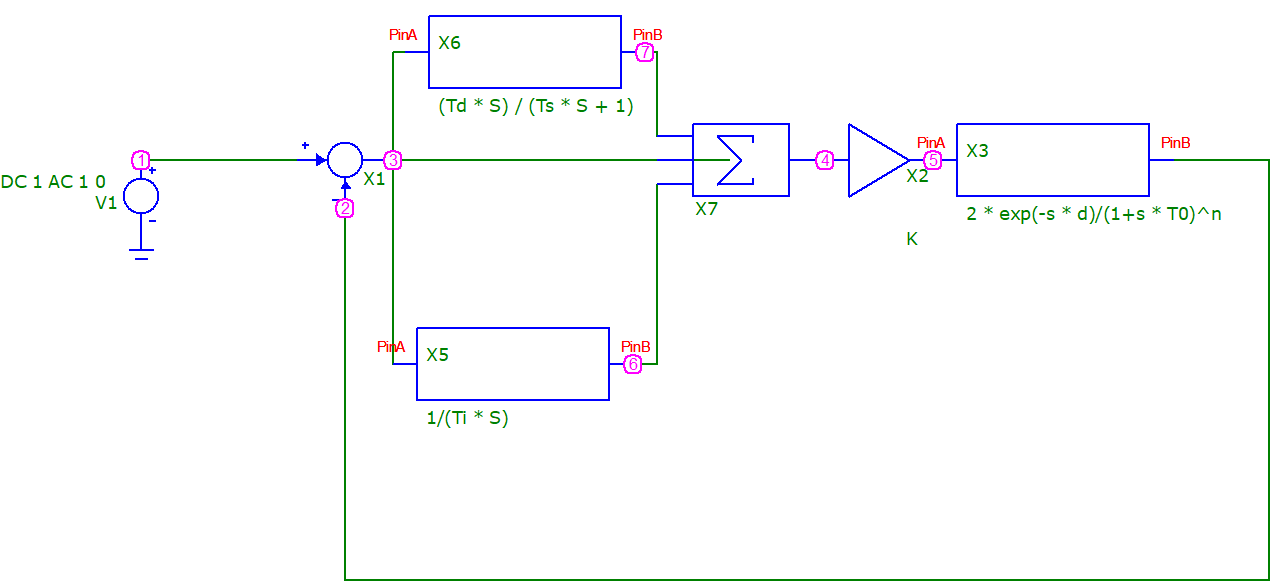
\includegraphics[scale=0.4]{./screens/schemes/pid_scheme.png}
	\caption{Схема ПИД-регулятора} 
\end{figure}

\begin{figure}[H]
	\centering
	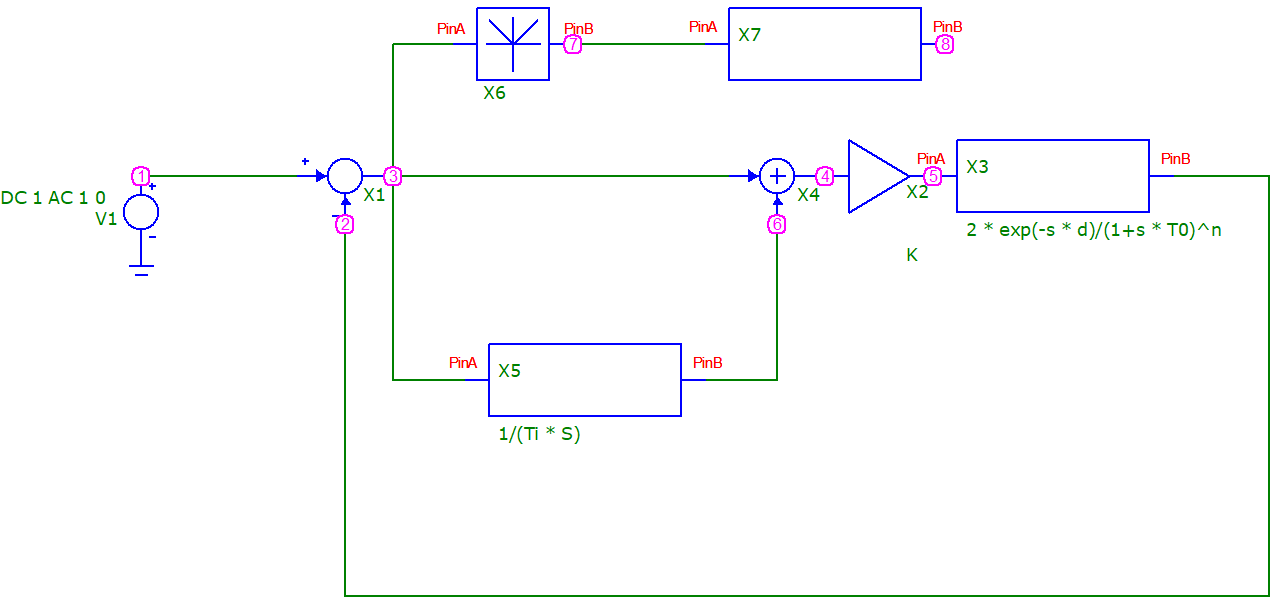
\includegraphics[scale=0.4]{./screens/schemes/pi_scheme_error.png}
	\caption{Схема ПИ-регулятора с вычислением интегральной ошибки} 
\end{figure}

\begin{figure}[H]
	\centering
	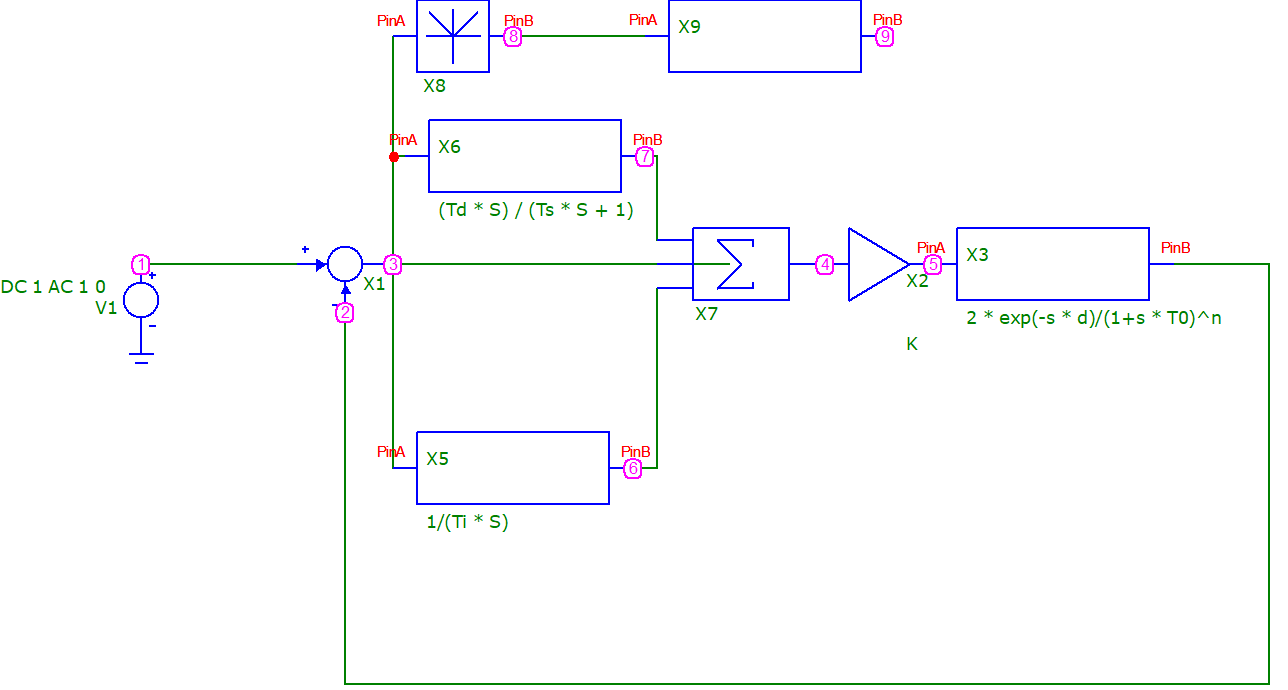
\includegraphics[scale=0.4]{./screens/schemes/pid_scheme_error.png}
	\caption{Схема ПИД-регулятора с вычислением интегральной ошибки} 
\end{figure}

\subsection{Разработка формул для настройки}
В ходе работы были разработаны формулы для параметров рассматриваемых объектов, которые должны минимизировать интегральную ошибку. Итоговые формулы имеют вид

\begin{center}
	\textbf{ПИ}
	\[K(T) = 0.7 e^{-0.24\sqrt{T}},\]
	\[T_i(T) = 4.9 e^{0.17\sqrt{T^3}};\]
\end{center}

\bigskip

\begin{center}
	\textbf{ПИД}
	\[K(T) = 0.932 e^{-0.15T^{\frac{5}{4}}},\]
	\[T_i(T) = 4 e^{0.195 T}.\]	
\end{center}

\bigskip

При разработке эти формул были сделаны 2 предположения, основанных на подборе параметров регуляторов:
\[\lim\limits_{T \to \infty} K(T) = 0, \quad \lim\limits_{T \to \infty} T_i(T) = +\infty,\]

также было сделано предположение о монотонности $K(T)$ и $T_i(T)$. В следствие этого были подобраны монотонные функции, которые бы проходили через точки, соответствующие настройкам регулятора через <<покоординатный спуск>>.

\begin{figure}[H]
	\centering
	\begin{tikzpicture}
		\begin{axis}[ 
			xmin=0, xmax=5,
			ymin=0, ymax=1,
			xlabel=$T$,
			ylabel={$K(T)$}
			] 
			\addplot [domain=0:5, color=blue, samples=1000] {0.7 * e^(-0.24 * sqrt(x))}; 
			\addplot [only marks] coordinates {
				(0, 0.6865)(1.5, 0.50875)(3, 0.48075)
			};
			\addlegendentry{$0.7 e^{-0.24\sqrt{T}}$}
		\end{axis}
	\end{tikzpicture}
	\caption{Разработанная зависимость $K(T)$ для ПИ-регулятора}
\end{figure}

\begin{figure}[H]
	\centering
	\begin{tikzpicture}
		\begin{axis}[ 
			xmin=0, xmax=5,
			ymin=0, ymax=40,
			xlabel=$T$,
			ylabel={$T_i(T)$},
			] 
			\addplot [domain=0:5, color=green, samples=1000] {4.9 * e^(0.17 * sqrt(x^3))};
			\addplot [only marks] coordinates {
				(0, 4.95583333333)(1.5, 6.7025)(3, 11.8363333333)
			}; 
			\addlegendentry{$4.9 e^{0.17\sqrt{T^3}}$}
		\end{axis}
	\end{tikzpicture}
	\caption{Разработанная зависимость $T_i(T)$ для ПИ-регулятора}
\end{figure}

\begin{figure}[H]
	\centering
	\begin{tikzpicture}
		\begin{axis}[ 
			xmin=0, xmax=5,
			ymin=0, ymax=1,
			xlabel=$T$,
			ylabel={$K(T)$}
			] 
			\addplot [domain=0:5, color=blue, samples=1000] {0.932 * e^(-0.15 * x^(5/4))}; 
			\addplot [only marks] coordinates {
				(0, 0.932)(1.5, 0.565)(3, 0.663)
			};
			\addlegendentry{$0.932 e^{-0.15T^{\frac{5}{4}}}$}
		\end{axis}
	\end{tikzpicture}
	\caption{Разработанная зависимость $K(T)$ для ПИД-регулятора}
\end{figure}			

\begin{figure}[H]
	\centering
	\begin{tikzpicture}
		\begin{axis}[ 
			xmin=0, xmax=5,
			ymin=0, ymax=15,
			xlabel=$T$,
			ylabel={$T_i(T)$},
			] 
			\addplot [domain=0:5, color=green, samples=1000] { 4 * e^(0.195 * x)};
			\addplot [only marks] coordinates {
				(0, 4.0035)(1.5, 5.4015)(3, 7.1035)
			}; 
			\addlegendentry{$4 e^{0.195 T}$}
		\end{axis}
	\end{tikzpicture}
	\caption{Разработанная зависимость $T_i(T)$ для ПИД-регулятора}
\end{figure}

\newpage

\section{Результаты моделирования и анализ результатов}
\begin{figure}[H]
	\centering
	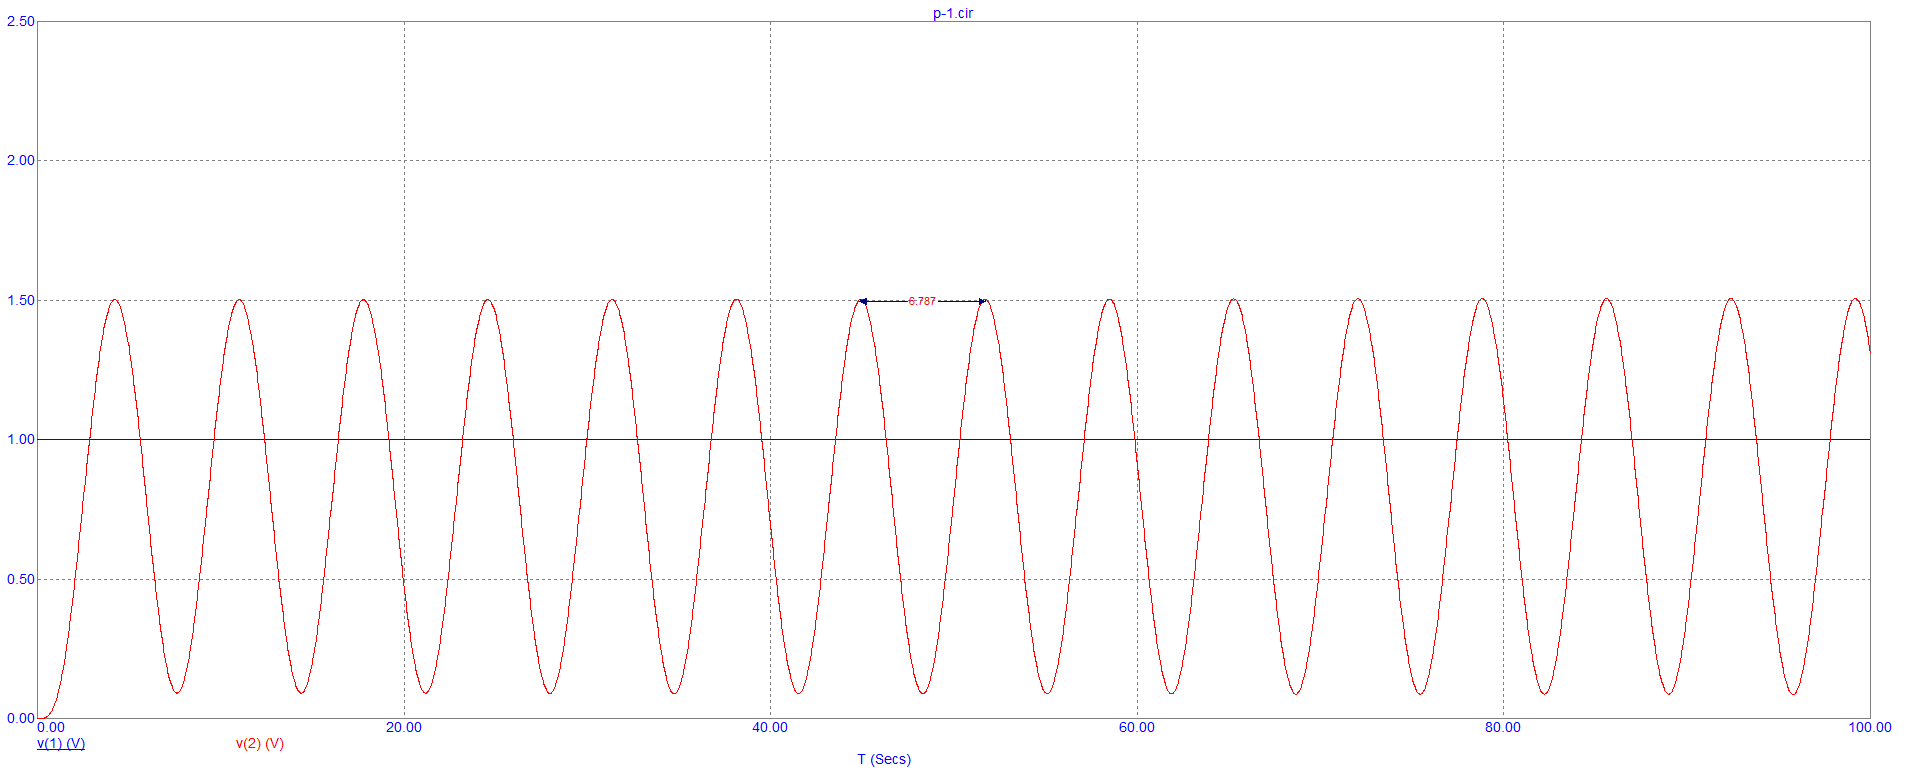
\includegraphics[scale=0.35]{./screens/plots/p_plot.png}
	\caption{Переходная характеристика П-регулятора в критическом режиме ($T = 0$, $K=K_{cr}=1.97$, $T_{cr}=6.787$)} 
\end{figure}

\begin{figure}[H]
	\centering
	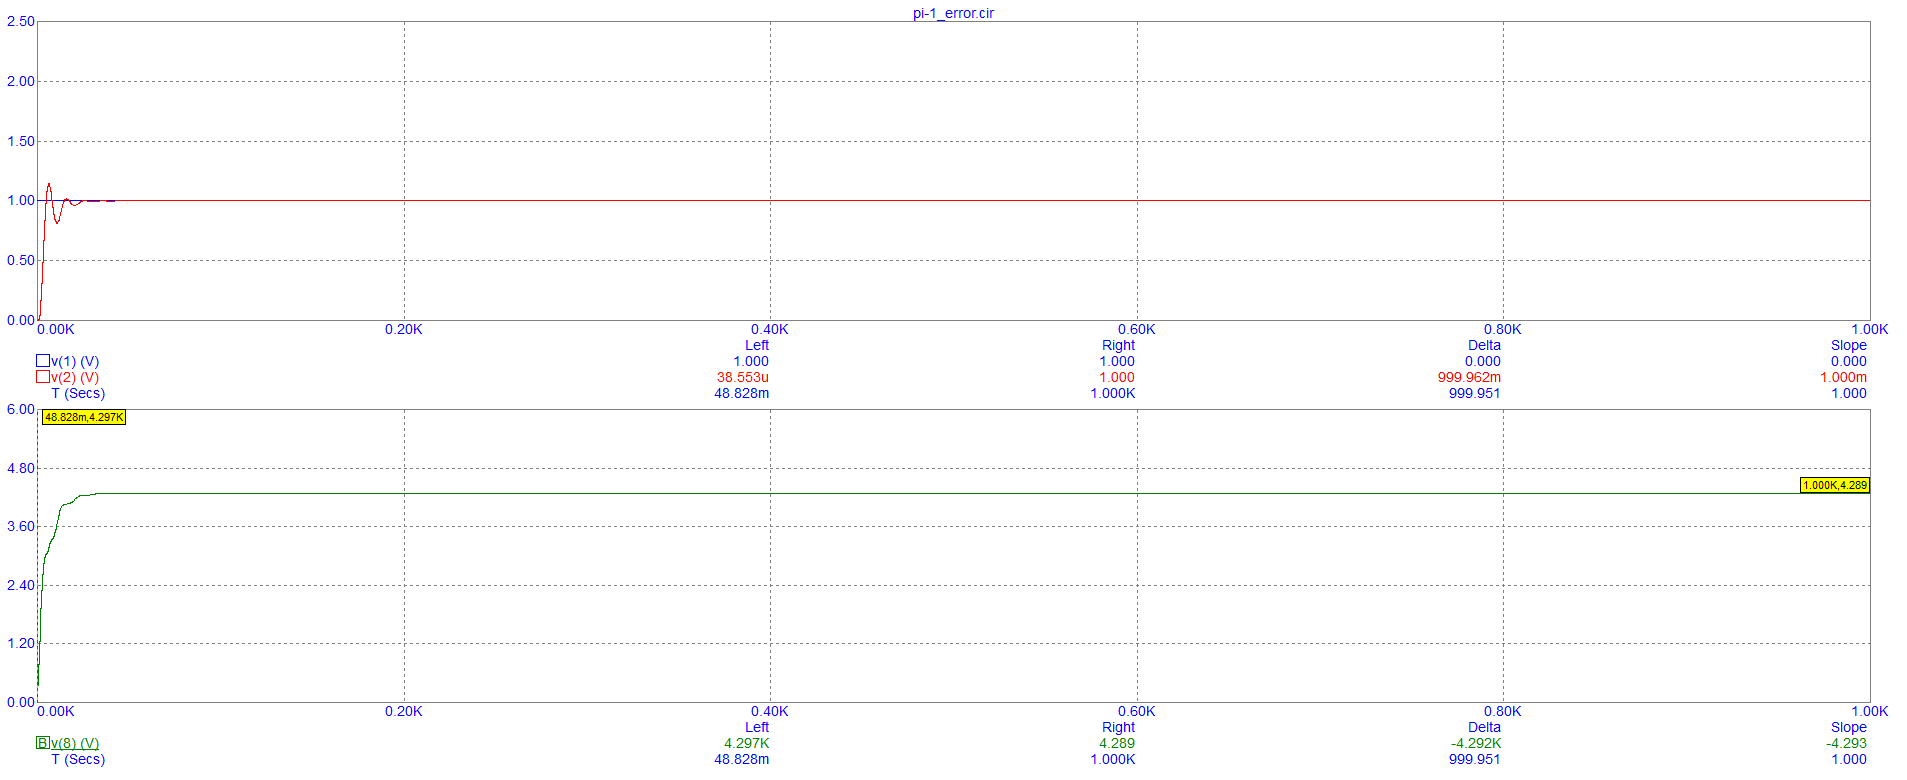
\includegraphics[scale=0.35]{./screens/plots/pi_plot_error.png}
	\caption{Переходная характеристика ПИ-регулятора вместе с интегральной ошибкой ($T = 0$, $K = 0.45Kcr - 0.2$, $Ti = Tcr / 1.2 - 0.7$)} 
\end{figure}

\begin{figure}[H]
	\centering
	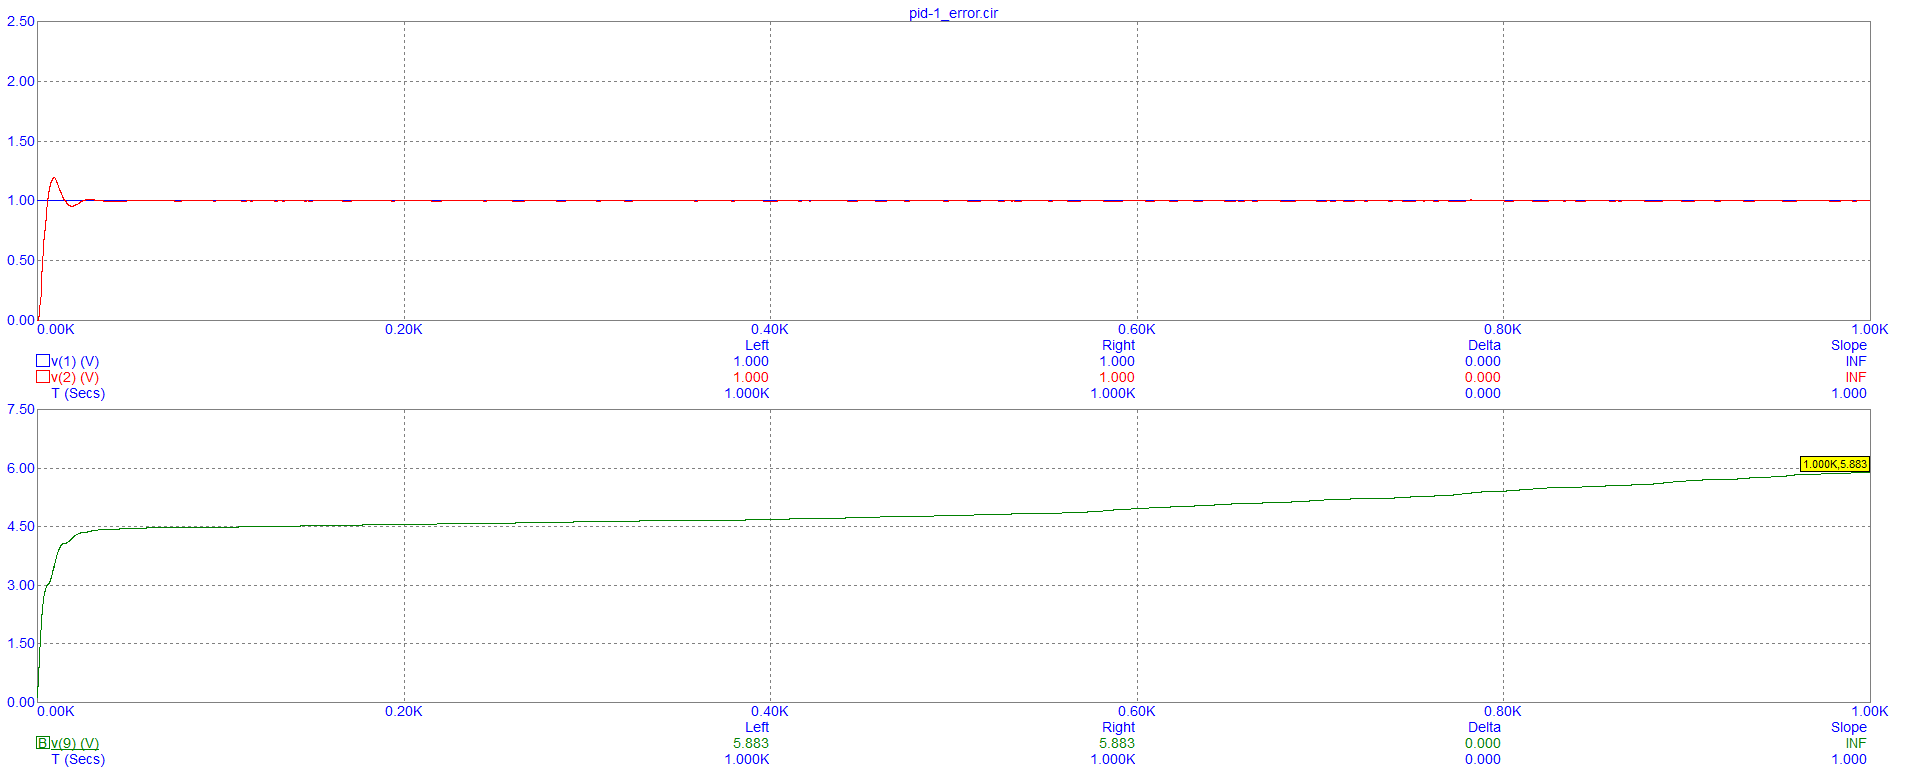
\includegraphics[scale=0.35]{./screens/plots/pid_plot_error.png}
	\caption{Переходная характеристика ПИД-регулятора вместе с интегральной ошибкой ($T = 0$, $K = 0.6K_{cr} - 0.25$, $T_i = T_{cr} / 2 + 0.61$, $Td = Ti / 4$, $Ts = Td / 8$)} 
\end{figure}

\newpage

\section{Выводы}
По ходу работы выяснилось, что при <<малых>> значениях задержки ($T < 3$) ПИ-регулятор даёт ошибку меньше, чем ПИД-регулятор, однако если задержка не является <<малой>> величиной, то ПИД-регулятор обеспечивает более хорошее качество регулирования. 

Также выяснилось, что использование готовых формул увеличивает интегральную ошибку по сравнению с <<покоординатным спуском>> и использованием формул, основанных на нём.

\begin{table}[H]
	\centering
	\begin{tabularx}{\textwidth}{
			| >{\arraybackslash}X
			| >{\arraybackslash}X
			|}
		\hline
		$\mathbf{T}$ & \textbf{Ошибка} \\\hline
		1 & 6.465\\\hline
		2 & 4.327\\\hline
		10 & 4.289\\\hline
	\end{tabularx}
	\caption{Интегральная ошибка ПИ-регулятора при использовании разработанных формул}
\end{table}

\bigskip

\begin{table}[H]
	\centering
	\begin{tabularx}{\textwidth}{
			| >{\arraybackslash}X
			| >{\arraybackslash}X
			|}
		\hline
		$\mathbf{T}$ & \textbf{Ошибка} \\\hline
		1 & 5.647\\\hline
		2 & 6.535\\\hline
		10 & 214.6\\\hline
	\end{tabularx}
	\caption{Интегральная ошибка ПИД-регулятора при использовании разработанных формул}
\end{table}

\bigskip	

\begin{table}[H]
	\centering
	\begin{tabularx}{\textwidth}{
			| >{\arraybackslash}X
			| >{\arraybackslash}X
			|}
		\hline
		$\mathbf{T}$ & \textbf{Ошибка} \\\hline
		1 & 66.517\\\hline
		2 & $\infty$\\\hline
		10 & 53.037\\\hline
	\end{tabularx}
	\caption{Интегральная ошибка ПИ-регулятора при использовании первого варианта готовых формул}
\end{table}

\bigskip

\begin{table}[H]
	\centering
	\begin{tabularx}{\textwidth}{
			| >{\arraybackslash}X
			| >{\arraybackslash}X
			|}
		\hline
		$\mathbf{T}$ & \textbf{Ошибка} \\\hline
		1 & $\infty$\\\hline
		2 & $\infty$\\\hline
		10 & 62.543\\\hline
	\end{tabularx}
	\caption{Интегральная ошибка ПИД-регулятора при использовании первого варианта готовых формул}
\end{table}

\bigskip

\begin{table}[H]
	\centering
	\begin{tabularx}{\textwidth}{
			| >{\arraybackslash}X
			| >{\arraybackslash}X
			|}
		\hline
		$\mathbf{T}$ & \textbf{Ошибка} \\\hline
		1 & 38.637\\\hline
		2 & 276\\\hline
		10 & $\infty$\\\hline
	\end{tabularx}
	\caption{Интегральная ошибка ПИ-регулятора при использовании второго варианта готовых формул}
\end{table}

\bigskip

\begin{table}[H]
	\centering
	\begin{tabularx}{\textwidth}{
			| >{\arraybackslash}X
			| >{\arraybackslash}X
			|}
		\hline
		$\mathbf{T}$ & \textbf{Ошибка} \\\hline
		1 & $\infty$\\\hline
		2 & $\infty$\\\hline
		10 & $\infty$\\\hline
	\end{tabularx}
	\caption{Интегральная ошибка ПИД-регулятора при использовании второго варианта готовых формул}
\end{table}

\newpage

\section{Приложения}
\begin{table}[h!]
	\centering
	\begin{tabularx}{\textwidth}{
			| >{\arraybackslash}X
			| >{\arraybackslash}X
			| >{\arraybackslash}X
			|}
		\hline
		$\mathbf{K}$ & $\mathbf{T_i}$ & \textbf{Ошибка}\\\hline
		$0.45 K_{cr}$ & $T_{cr} / 1.2$ & $4.928$\\\hline
		$0.45 K_{cr} - 0.15$ & $T_{cr} / 1.2 - 0.35$ & $4.327$\\\hline
		$0.45 K_{cr} - 0.2$ & $T_{cr} / 1.2 - 0.7$ & $4.289$\\\hline
	\end{tabularx}
	\caption{Итеративный процесс нахождения оптимальных характеристик ПИ-регулятора при $T = 0$}
\end{table}

\bigskip

\begin{table}[h!]
	\centering
	\begin{tabularx}{\textwidth}{
			| >{\arraybackslash}X
			| >{\arraybackslash}X
			| >{\arraybackslash}X
			|}
		\hline
		$\mathbf{K}$ & $\mathbf{T_i}$ & \textbf{Ошибка}\\\hline
		$0.6 K_{cr}$ & $T_{cr} / 2$ & $8.341$\\\hline
		$0.6 K_{cr} - 0.31$ & $T_{cr} / 2 + 0.5$ & $6.924$\\\hline
		$0.6 K_{cr} - 0.25$ & $T_{cr} / 2 + 0.61$ & $5.883$\\\hline
	\end{tabularx}
	\caption{Итеративный процесс нахождения оптимальных характеристик ПИД-регулятора при $T = 0$}
\end{table}

\bigskip

\begin{table}[h!]
	\centering
	\begin{tabularx}{\textwidth}{
			| >{\arraybackslash}X
			| >{\arraybackslash}X
			| >{\arraybackslash}X
			|}
		\hline
		$\mathbf{K}$ & $\mathbf{T_i}$ & \textbf{Ошибка}\\\hline
		$0.45 K_{cr}$ & $T_{cr} / 1.2$ & $10.260$\\\hline
		$0.45 K_{cr} + 0.11$ & $T_{cr} / 1.2 - 1.4$ & $8.232$\\\hline
		$0.45 K_{cr} + 0.07$ & $T_{cr} / 1.2 - 2.3$ & $7.742$\\\hline
	\end{tabularx}
	\caption{Итеративный процесс нахождения оптимальных характеристик ПИ-регулятора при $T = 1.5$}
\end{table}

\bigskip

\begin{table}[h!]
	\centering
	\begin{tabularx}{\textwidth}{
			| >{\arraybackslash}X
			| >{\arraybackslash}X
			| >{\arraybackslash}X
			|}
		\hline
		$\mathbf{K}$ & $\mathbf{T_i}$ & \textbf{Ошибка}\\\hline
		$0.6 K_{cr}$ & $T_{cr} / 2$ & $6.529$\\\hline
		$0.6 K_{cr} - 0.01$ & $T_{cr} / 2 + 0.01$ & $6.346$\\\hline
		$0.6 K_{cr} - 0.02$ & $T_{cr} / 2$ & $6.345$\\\hline
	\end{tabularx}
	\caption{Итеративный процесс нахождения оптимальных характеристик ПИД-регулятора при $T = 1.5$}
\end{table}

\bigskip

\begin{table}[h!]
	\centering
	\begin{tabularx}{\textwidth}{
			| >{\arraybackslash}X
			| >{\arraybackslash}X
			| >{\arraybackslash}X
			|}
		\hline
		$\mathbf{K}$ & $\mathbf{T_i}$ & \textbf{Ошибка}\\\hline
		$0.45 K_{cr}$ & $T_{cr} / 1.2$ & $17.427$\\\hline
		$0.45 K_{cr} + 0.14$ & $T_{cr} / 1.2 - 0.005$ & $12.932$\\\hline
		$0.45 K_{cr} + 0.141$ & $T_{cr} / 1.2 - 0.0045$ & $12.929$\\\hline
	\end{tabularx}
	\caption{Итеративный процесс нахождения оптимальных характеристик ПИ-регулятора при $T = 3$}
\end{table}

\bigskip

\begin{table}[h!]
	\centering
	\begin{tabularx}{\textwidth}{
			| >{\arraybackslash}X
			| >{\arraybackslash}X
			| >{\arraybackslash}X
			|}
		\hline
		$\mathbf{K}$ & $\mathbf{T_i}$ & \textbf{Ошибка} \\\hline
		$0.6 K_{cr}$ & $T_{cr} / 2$ & $8.765$\\\hline
		$0.6 K_{cr} + 0.2$ & $T_{cr} / 2 - 0.0001$ & $7.626$\\\hline
		$0.6 K_{cr} + 0.21$ & $T_{cr} / 2 - 0.0001$ & $7.574$\\\hline
	\end{tabularx}
	\caption{Итеративный процесс нахождения оптимальных характеристик ПИД-регулятора при $T = 3$}
\end{table}
